\documentclass[numbers=noendperiod]{scrartcl}
\usepackage[utf8]{luainputenc}
\usepackage[T1]{fontenc}
\usepackage[ngerman]{babel}
\usepackage[a4paper,margin=0.75in, bottom=1in]{geometry}
\usepackage{enumerate}
\usepackage{minted}
\usepackage{mdframed}
\usepackage{courier}
\usepackage{hyperref}
\usepackage{graphicx}
\usepackage{subcaption}
\usepackage{amsmath}
\begin{document}
	
	\setlength{\parindent}{0em} 
	
	\definecolor{bg}{RGB}{230,230,230}
	\newcommand{\inputmintedframed}[2]{
		\begin{mdframed}[linecolor=bg,backgroundcolor=bg]
			\inputminted[mathescape,breaklines,linenos,numbersep=5pt,tabsize=3]{#1}{#2}
	\end{mdframed}}
	
	\hrulefill
	\begin{center}
		\bfseries % Fettdruck einschalten
		\sffamily % Serifenlose Schrift
		\begin{huge}
			Betriebs- und Kommunikationssysteme
		\end{huge}\\
		\begin{Large}
			Sommersemester 2017, 9. Übungsblatt
		\end{Large}\\
		\begin{small}
			Christoph Husemann, Luis Herrmann; Tutor: André Schröder; Mi 16:00-18:00
		\end{small}
		
		\vspace{-10pt}
	\end{center}
	\hrulefill
	
\section*{Aufgabe 1}
\subsection*{a) Aufgaben des Data-Link-Layers (Sicherungsschicht)}
Data-Link-Layers bekommen als 2-Schicht von den physical-Layers (Schicht 1) (Bit-Übertragungsschicht) einen Strom von Bits und IP-Pakete von dem Network layer(Schicht 3). Die Aufgaben des Data-Link-Layers sind insbesondere:
\begin{enumerate}
	\item Fehler erkennen und korrigieren
	\item Transparente Übertragung von Daten
	\item Rahmen (Frames)
	\begin{enumerate}
		\item Rahmen für Bitstreams zum physical-layer bilden
		\item Rahmen in Bitstreams des Network layers erkennen 
		\item Trailer mit Prüfsumme (Frame check sequence FCS) und ggfl. Header hinzufügen
		\item Bitstuffing der Nutzdaten via Hardware, um Flags für den Rahmen von Nutzdaten zu unterscheiden
	\end{enumerate}
	\item Ermitteln der best möglichen Übertragungsgeschwindigkeit zum nächsten Host (z.B. Router) (Flow control)
	\item Verbindung zum Host aufbauen/schließen
	
\end{enumerate}
\subsection*{b) Angabe des Bitstrings der Ascii-Zeichen ''?~''}
Ascii Wert von ? ist: 0x3F = 0011 1111 \\
Ascii Wert von ~ ist: 0x7E = 0111 1110 \\
\(\Rightarrow \) der Bitstring der Ascii-Zeichen ''?~'' lautet ''0011 1111 0111 1110''
\subsubsection*{Ergänzung um die CRC16 Prüfsumme}
Das CRC16 IBM Prüfpolynom lautet \(x^{16}+x^{15}+x^2 + 1 \Rightarrow \) 1 1000 0000 0000 0101 \\ \\
  \begin{tabular}{cl}
&11 1111 0111 1110 0000 0000 0000 0000 \ / \ 1 1000 0000 0000 0101 = 10101001010100\\
&\underline{11 0000 0000 0000 101}\\
   &\phantom{00 }1111 0111 1110 1010 0\\
   &\phantom{00 }\underline{1100 0000 0000 0010 1}\\
     &\phantom{00 00}11 0111 1110 1000 100\\
	 &\phantom{00 00}\underline{11 0000 0000 0000 101}\\
		&\phantom{00 0000 }0111 1110 1000 0010 00\\
		 &\phantom{00 0000 0}\underline{110 0000 0000 0001 01}\\
		   &\phantom{00 0000 000}1 1110 1000 0011 0100\\
		   &\phantom{00 0000 000}\underline{1 1000 0000 0000 0101}\\
		      &\phantom{00 0000 0000 0}110 1000 0011 0001 00\\
		      &\phantom{00 0000 0000 0}\underline{110 0000 0000 0001 01}\\
		          &\phantom{00 0000 0000 0000 }1000 0011 0000 0100\\
		        \end{tabular}\\ \\
		        \(\Rightarrow\) CRC16 Prüfsumme ist 1000 0011 0000 0100\\
		        \(\Rightarrow\) Bitstring:0011 1111 0111 1110 1000 0011 0000 0100
\subsubsection*{Bistuffing}
Immer nach fünf Einerbits hintereinander wird eine Null eingefügt
 \(\Rightarrow\) Bitstring: 0011 111\textbf{0}1 0111 11\textbf{0}10 1000 0011 0000 0100
\subsubsection*{Manchester Codierung}
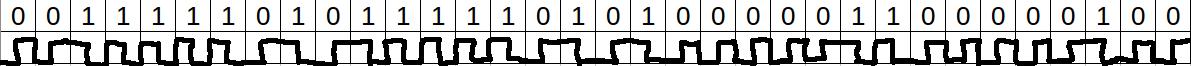
\includegraphics[width=1.0\textwidth]{manchester.png}
\subsubsection*{Amplitudenmodulation}
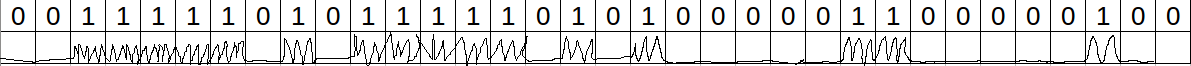
\includegraphics[width=1.0\textwidth]{amplitude.png}
\section*{Aufgabe 2}

\subsection*{a + c}

\inputmintedframed{c}{crc.c}

\subsection*{c}
Für die ersten 17-Bit unserer ersten Datei (gen1) wählen wir die bitweise Negation des Polynoms und ''füllen'' das letzte Byte mit Nullen und am Schluss einer 1 auf. \\ \\

001111111111110100000001 \(\Rightarrow \) 0x3f 0xfd 0x01 \(\Rightarrow \) 0x8D05 \\ \\
Für die zweite Datei nehmen wir die erste Datei (gen2) und führen ein bitweises xor mit dem Polynom auf den ersten 17-Bits aus und erhalten so 17 mal die 1. Da im ersten Schritt der Polynomdivision auf der zweiten Datei ein xor auf den ersten 17-Bits ausgeführt wird, erhalten wir diesem Schritt die erste Datei. Da der CRC-Hash nur der Rest der Polynomdivision ist, sind die Hashes identisch.\\ \\

111111111111111110000001 \(\Rightarrow \) 0xff 0xff 0x81 \(\Rightarrow \) 0x8D05 \\ \\


\end{document}
